\providecommand{\main}{../../../..}
\documentclass[\main/dresen_thesis.tex]{subfiles}
\renewcommand{\thisPath}{\main/chapters/theoreticalBackground/scattering/sas}
\begin{document}
  \subsection{Small-Angle Scattering from Nanoparticles}\label{sec:theoreticalBackground:scattering:SASNanoparticles}
    Small-angle scattering is a technique to study nanometer sized objects when the wavelength of the scattered particle is in the order of a few {\aa}ngstr\"om.
    Here, the forward scattering of a collimated beam through a sample is measured on a position sensitive detector around an opening angle in the order of $2 \theta \eq 0.1^\circ - 10^\circ$.
    As the magnitude of the scattering vector $q$ is proportional to $\sin(\theta)$ and $q$ is inversely proportional to the probed length scale, smaller scattering angles $\theta$ mean that larger length scales are probed.
    At the considered length scales, the atomic structure of the materials can be treated in the continuum limit as described in \refsec{sec:theoreticalBackground:scattering:interactionWithMatter}.

    \begin{figure}[tb]
      \centering
      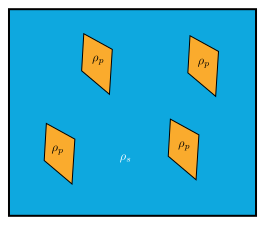
\includegraphics{scatteringTheory_sasParticlesInSolvent}
      \caption{\label{fig:theoreticalBackground:scattering:scatteringTheory:sasParticlesInSolvent}Scattering length density described in \refeq{eq:theoreticalBackground:scattering:scatteringTheory:sasParticlesInSolvent}. The space is completely filled with the solvent $\rho_s$ and at positions of the nanoparticles the solvent is replaced by the scattering length density function describing a nanoparticle $\rho_p$.}
    \end{figure}
    In the following, the application of small-angle scattering to the study of nanoparticles in dispersion is described.
    In a first step, a dispersion that consists of monodisperse and equally oriented nanoparticles is considered.
    In this case the scattering length density is modeled by a constant background value given by the solvent $\rho_s$ and parts where the solvent is replaced by the nanoparticles.
    As every particle is equally oriented and of same shape, this is included by summing over a function $\rho_p (\vec{r})$ that contains the complete description of shape and composition of a single particle and which is shifted to the different center positions $\vec{r}_i$ of the nanoparticles
    \begin{align}
      \rho(\vec{r}) \eq& \rho_s + \sum_{i=1}^N \Delta \rho_{p}(\vec{r} - \vec{r}_i).\label{eq:theoreticalBackground:scattering:scatteringTheory:sasParticlesInSolvent}
    \end{align}
    The nanoparticle scattering length density can be written as convolution of the function $\Delta \rho_{p}(\vec{r})$, which describes the shape and composition of a single nanoparticle, and a function $s(\vec{r})$ describing the position of $N$ nanoparticles in the solvent\footnote{The convolution of two functions is defined as $(f*g)(x) \eq \int \dint \tau f(\tau) g(x-\tau)$.
    When $f$ is a sum over $\delta$ functions, the convolution operation generates a sum of the function $g$, centered at every grid point defined by the $\delta$ functions
    \begin{equation}
      \int \dint \tau \sum_{i=1}^N \delta(\tau - x_i) g(x-\tau) \eq \sum_{i=1}^N g(x - x_i).
    \end{equation}}
    \begin{align}
      \rho(\vec{r}) \eq& \rho_s + (s * \Delta \rho_{p})(\vec{r}),\\
      s(\vec{r}) \eq& \sum_{j=1}^N \delta(\vec{r} - \vec{r}_j).
    \end{align}

    The macroscopic differential cross section, which is the differential cross section scaled to the integrated volume
    \begin{align}
      \frac{\dint \Sigma}{\dint \Omega} \eq \frac{1}{V} \frac{\dint \sigma}{\dint \Omega},
    \end{align}
    can then be evaluated in the Born approximation by inserting the scattering length density in \refeq{eq:theoreticalBackground:scattering:scatteringTheory:differentialCrossSectionBornApproximation}
    \begin{align}
      \begin{split}
        \frac{\dint \Sigma}{\dint \Omega}
        \eq& \frac{1}{V} \bigg| \int_V \dint \vec{r}^\prime e^{-i\vec{q} \cdot \vec{r}^\prime} \rho (\vec{r}^\prime) \bigg|^2 \\
        \eq& \frac{1}{V} \bigg| \int_{V} \dint \vec{r}^\prime e^{-i\vec{q} \cdot \vec{r}^\prime} \biggl( s * \Delta \rho_{p}) \biggr) (\vec{r}^\prime) + \underbrace{\int_{V} \dint \vec{r}^\prime e^{-i\vec{q} \cdot \vec{r}^\prime} \rho_s }_{(2 \pi)^3 \delta(\vec{q}) \rho_s} \bigg|^2.
      \end{split}
    \end{align}
    The integral over the constant solvent scattering length density is evaluated to zero for $\vec{q} \neq 0$.
    The case of $\vec{q} \eq 0$ corresponds to forward scattering, which is not studied in small-angle scattering as the direct beam is in most experiments blocked to protect the detector.

    The convolution theorem turns the remaining integral to a product of two integrals
    \begin{align}
      \frac{\dint \Sigma}{\dint \Omega}
      \eq \frac{N}{V} \underbrace{\frac{1}{N} \bigg|\int \dint \vec{r} e^{-i\vec{q} \cdot \vec{r}} s(\vec{r})\bigg|^2}_{S(\vec{q})}
      \underbrace{ \bigg|\int_{V_{p}} \dint \vec{r} e^{-i\vec{q} \cdot \vec{r}} (\rho_p (\vec{r}) - \rho_s) \bigg|^2}_{P(\vec{q})},\label{eq:theoreticalBackground:scattering:scatteringTheory:sasParticlesformStructureFactor}
    \end{align}
    The first integral is called the structure factor $S(\vec{q})$ and the second the form factor $P(\vec{q})$.
    The form factor describes the scattering due to the shape and properties of a single nanoparticle.
    In the definition of the volume integral for the form factor, it is enough to integrate over the volume of a single particle $V_p$ as the integrand is $0$ outside, and $\Delta \rho_p (\vec{r})$ is explicitly written.
    The integral, before applying the magnitude square, is called the form factor amplitude and is denoted by a lower case $p(\vec{q})$.
    As the magnitude removes the phase of the amplitude, it's in general hard to revert the integration and conclude from the differential cross section directly on the shape and composition of the nanoparticle due to the missing information.
    Using additional information from multiple experiments a model can, however, be formulated for a particle and from this the form factor can always be calculated, which is compared to the small-angle scattering experiment for confirmation.

    The structure factor in \refeq{eq:theoreticalBackground:scattering:scatteringTheory:sasParticlesformStructureFactor} modulates the scattering due to the relative positions of the ensemble of individual nanoparticles.
    It is normalized to the number of particles $N$ for proper scaling behaviour and can generally be further discussed by inserting the definition of the function $s(\vec{r})$
    \begin{align}
      \begin{split}
        S(\vec{q}) &\eq \frac{1}{N} \bigg| \sum_j  e^{-i\vec{q} \cdot \vec{r}_j} \bigg|^2\\
        &\eq \frac{1}{N}  \bigg( \sum_j  e^{-i\vec{q} \cdot \vec{r}_j} \bigg) \bigg( \sum_k  e^{i k\vec{q} \cdot \vec{r}_k} \bigg)\\
        &\eq \frac{1}{N}  \sum_{j, k}  e^{-i\vec{q} \cdot (\vec{r}_j - \vec{r}_k) }\\
        &\eq 1 + \frac{1}{N}  \sum_{j \neq k}  e^{-i\vec{q} \cdot (\vec{r}_j - \vec{r}_k)},\label{eq:theoreticalBackground:scattering:scatteringTheory:structureFactor}
      \end{split}
    \end{align}
    where in the last step the sum over all indices, where $j=k$, was performed.
    At this point, specific models of the relative nanoparticle positions needs to be looked at for further discussion.

    The simplest models that can be solved are perfectly ordered crystals and disordered liquids.
    For ordered crystals, constructive contributions are found when $\vec{q} \cdot (\vec{r}_j - \vec{r}_k) \eq 2 \pi n$, which is Bragg's law in this frame.
    In the case of dilute dispersions, the sum is over random phases and vanishes due to the prefactor, resulting in $S(\vec{q}) = 1$.
    This case is most often the desired one in a small-angle scattering experiment on nanoparticles as it eliminates the need to model a structure factor.
    Therefore, in a experiment, the sample is diluted such that the structure factor is approximately $1$, but the measured intensity is still strong enough to be counted in a reasonable amount of measurement time.
    In this case, only the form factor $P(\vec{q})$ for a specific sample needs to be modeled

    For a form factor, the simplest to solve model of a nanoparticle is that of a sphere due to it's high symmetry.
    The scattering length density is then just a constant within the volume of the sphere and the form factor $P_\mathrm{sph}$ can be solved analytically to
    \begin{align}
      \begin{split}
        P_\mathrm{sph} (\vec{q})
        \eq & \bigg|\int_{V_{p}} \dint \vec{r} e^{-i\vec{q} \cdot \vec{r}} (\rho_p - \rho_s) \bigg|^2 \\
        \eq & \bigg|(\rho_p - \rho_s) \int_0^R \dint r \int_0^{2 \pi} \dint \phi \int_0^\pi \dint \theta r^2 \sin(\theta) e^{-i q r \cos(\theta)}  \bigg|^2 \\
        \eq &  \bigg| 4\pi R^3 (\rho_p - \rho_s) \frac{\sin(qR) - qR\cos(qR)}{(qR)^3}  \bigg|^2\\
        \eq & V_\mathrm{sph}^2 (\rho_p - \rho_s)^2 \bigg|3 \frac{\sin(qR) - qR\cos(qR)}{(qR)^3}  \bigg|^2,
      \end{split}
    \end{align}
    where $V_\mathrm{sph}$ is the volume of the sphere.
    Thus, the macroscopic differential cross section for diluted nanospheres in a solvent is
    \begin{align}
      \frac{\dint \Sigma}{\dint \Omega}
      \eq \alpha V_\mathrm{sph} (\rho_p - \rho_s)^2 \bigg|3 \frac{\sin(qR) - qR\cos(qR)}{(qR)^3}  \bigg|^2,
    \end{align}
    with $\alpha \eq NV_\mathrm{sph} / V$ the volume concentration of the particles in the solvent.
    The result shows the typical dependence of the differential cross section on the particle concentration, volume and contrast to the solvent.
    The latter is especially used for contrast variation techniques in neutron scattering, where solvents (especially $\mathrm{H_2O}$ and $\mathrm{D_2O}$) are mixed to tune the scattering length density of the solvent to enhance the signal or mask particles.
    The derivation of further form factors used in this work such as a cube or superball, and how to include multiple compositions in a core shell model is further elaborated in \refapp{sec:appendix:formfactors}.
    As will become evident in the following work, small-angle scattering is a very powerful technique to characterize a large number of particles in a sample, and the obtained results are valuable in evaluating higher order experiments which rely on the characterized samples.
\end{document}